\documentclass[11pt]{article}

% ======================================================================
%  Dobbertin (1999) — structural patterns, told in pictures
%  A lightweight, visual companion to the RequestProject formalisation.
%  Little prose, many diagrams.  Compile with:  tectonic DobbertinPatterns.tex
% ======================================================================

\usepackage[a4paper,margin=2.2cm]{geometry}
\usepackage{amsmath,amssymb}
\usepackage{tikz}
\usepackage{xcolor}
\usepackage{enumitem}
\usepackage{hyperref}
\hypersetup{colorlinks=true,linkcolor=blue!55!black,urlcolor=teal!60!black}

\usetikzlibrary{arrows.meta,positioning,calc,fit,backgrounds,shapes.geometric,
                shapes.misc,decorations.pathmorphing,decorations.pathreplacing,
                shadows.blur}

% ---- palette ----------------------------------------------------------
\definecolor{cKas}{HTML}{1B6CA8}   % Kasami blue
\definecolor{cMcm}{HTML}{B5495B}   % MCM red
\definecolor{cDs} {HTML}{2E8B57}   % difference-set green
\definecolor{cFour}{HTML}{8250C4}  % Fourier purple
\definecolor{cGold}{HTML}{C98A00}  % gold/frobenius
\definecolor{cInk}{HTML}{22303A}
\definecolor{cPaper}{HTML}{F6F4EE}

% ---- reusable node styles --------------------------------------------
\tikzset{
  >=Stealth,
  box/.style   ={rounded corners=3pt,draw=cInk,fill=cPaper,
                 align=center,inner sep=5pt,font=\small},
  kbox/.style  ={box,draw=cKas,fill=cKas!8,text=cInk},
  mbox/.style  ={box,draw=cMcm,fill=cMcm!8,text=cInk},
  dbox/.style  ={box,draw=cDs, fill=cDs!8, text=cInk},
  fbox/.style  ={box,draw=cFour,fill=cFour!8,text=cInk},
  gbox/.style  ={box,draw=cGold,fill=cGold!12,text=cInk},
  dot/.style   ={circle,fill=cInk,inner sep=1.5pt},
  ar/.style    ={->,thick,cInk},
  arb/.style   ={->,very thick},
  lbl/.style   ={font=\footnotesize\itshape,fill=cPaper,inner sep=1.5pt},
}

\newcommand{\GF}{\mathbb{F}}
\newcommand{\Tr}{\operatorname{Tr}}
\newcommand{\gcdt}{\gcd}
\newcommand{\dk}{d_k}

\title{\bfseries The Dobbertin (1999) Kasami paper,\\ told in pictures}
\author{\normalsize A visual map of the structural patterns\\
\normalsize and how they propagate through the theorems}
\date{\normalsize companion to \texttt{RequestProject/} \;($\!$every claim below is a \texttt{sorry}-free Lean fact$)$}

\begin{document}
\maketitle
\thispagestyle{empty}

\begin{center}
\footnotesize
\emph{H.\ Dobbertin, ``Kasami Power Functions, Permutation Polynomials and Cyclic
Difference Sets'', NATO Sci.\ Ser.\ C \textbf{542}, Kluwer, 1999.}\\[2pt]
Field $L=\GF_{2^n}$,\quad Kasami exponent $\dk = 2^{2k}-2^{k}+1$,\quad
$\gcd(k,n)=1$.
\end{center}

\vspace{2pt}
\hrule
\vspace{6pt}

% ======================================================================
\section*{1.\quad The paper in one picture: three pillars, one spine}
% ======================================================================
\noindent\emph{Simple English:} the title names three things. They are held up by
a single chain of arrows. Follow the thick arrows.

\begin{center}
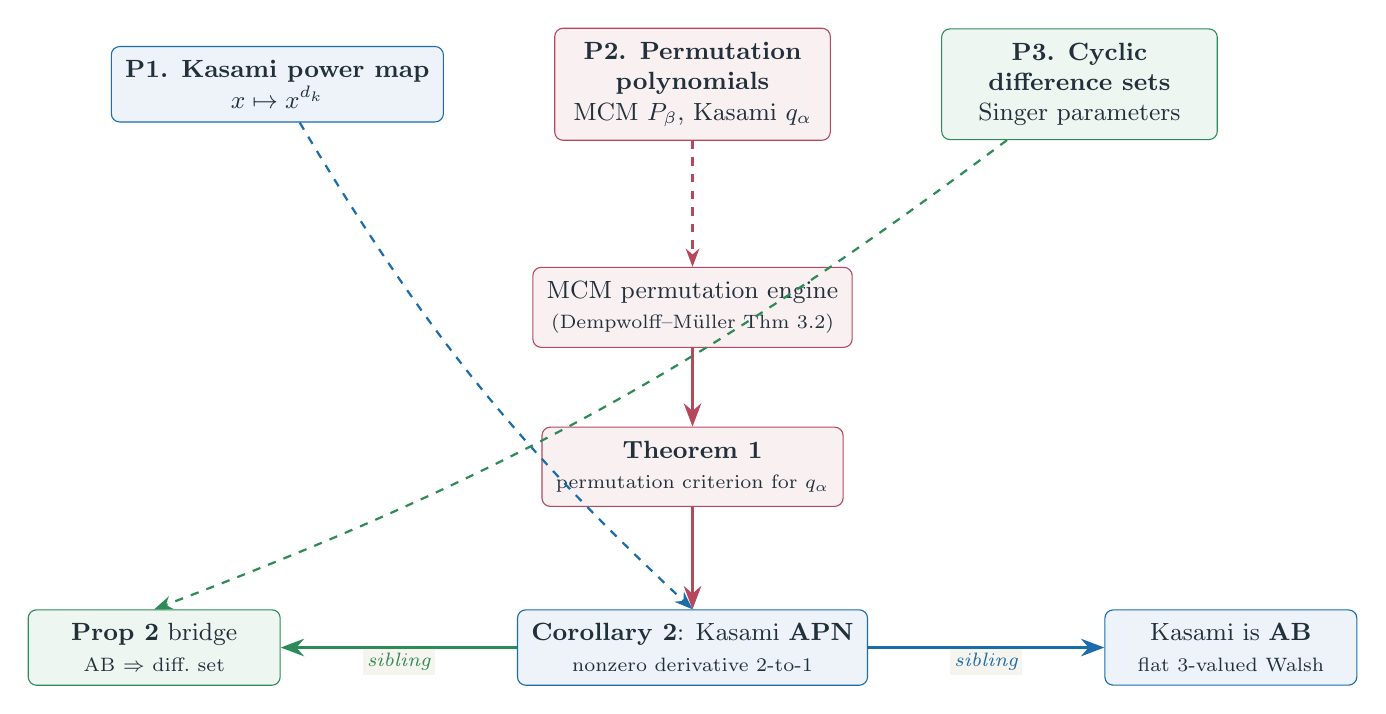
\begin{tikzpicture}[node distance=8mm]
% pillars header
\node[kbox,minimum width=3.5cm] (p1) {\textbf{P1. Kasami power map}\\ $x\mapsto x^{\dk}$};
\node[mbox,right=14mm of p1,minimum width=3.5cm] (p2) {\textbf{P2. Permutation}\\ \textbf{polynomials}\\ MCM $P_\beta$, Kasami $q_\alpha$};
\node[dbox,right=14mm of p2,minimum width=3.5cm] (p3) {\textbf{P3. Cyclic}\\ \textbf{difference sets}\\ Singer parameters};

% spine below
\node[mbox,below=16mm of p2] (eng) {MCM permutation engine\\ \scriptsize(Dempwolff--M\"uller Thm 3.2)};
\node[mbox,below=10mm of eng] (t1) {\textbf{Theorem 1}\\ \scriptsize permutation criterion for $q_\alpha$};
\node[kbox,below=13mm of t1,minimum width=3.4cm] (c2) {\textbf{Corollary 2}: Kasami \textbf{APN}\\ \scriptsize nonzero derivative $2$-to-$1$};
\node[kbox,right=30mm of c2,minimum width=3.2cm] (ab) {Kasami is \textbf{AB}\\ \scriptsize flat 3-valued Walsh};
\node[dbox,left=30mm of c2,minimum width=3.2cm] (ds) {\textbf{Prop 2} bridge\\ \scriptsize AB $\Rightarrow$ diff.\ set};

\draw[arb,cMcm] (eng)--(t1);
\draw[arb,cMcm] (t1)--(c2);
\draw[arb,cKas] (c2)--(ab) node[lbl,midway,below]{\scriptsize sibling};
\draw[arb,cDs]  (c2)--(ds) node[lbl,midway,below]{\scriptsize sibling};

\draw[ar,dashed,cKas] (p1) to[bend right=8] (c2.north);
\draw[ar,dashed,cMcm] (p2) -- (eng);
\draw[ar,dashed,cDs]  (p3) to[bend left=8] (ds.north);
\end{tikzpicture}
\end{center}

\begin{center}\footnotesize
\fbox{\parbox{0.86\textwidth}{\centering
The spine: \textcolor{cMcm}{\textbf{MCM permutation engine}} $\to$
\textcolor{cMcm}{\textbf{Theorem 1}} $\to$
\textcolor{cKas}{\textbf{Corollary 2 (APN)}}.\\
Everything else hangs off Corollary~2 as a Fourier-side twin.}}
\end{center}

\newpage
% ======================================================================
\section*{2.\quad The one big idea: work on the Fourier side}
% ======================================================================
\noindent\emph{Simple English:} a hard property of a \emph{map} becomes an easy
property of its \emph{Walsh transform}. ``Hard, multiplicative'' turns into
``flat'' or ``zero''.

\begin{center}
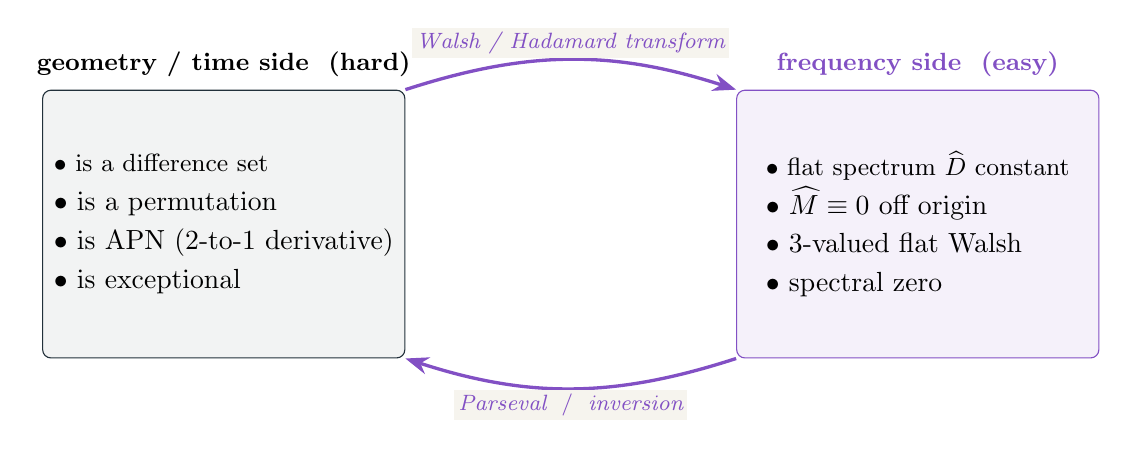
\begin{tikzpicture}
% left: hard side
\node[box,fill=cInk!6,minimum width=4.6cm,minimum height=3.4cm] (L) {};
\node[above=1pt of L.north,font=\small\bfseries] {geometry / time side\ \ (hard)};
\node[align=left] at (L) {
  \small
  $\bullet$ is a difference set\\[2pt]
  $\bullet$ is a permutation\\[2pt]
  $\bullet$ is APN ($2$-to-$1$ derivative)\\[2pt]
  $\bullet$ is exceptional
};

% right: easy side
\node[fbox,minimum width=4.6cm,minimum height=3.4cm,right=42mm of L] (R) {};
\node[above=1pt of R.north,font=\small\bfseries,text=cFour] {frequency side\ \ (easy)};
\node[align=left] at (R) {
  \small
  $\bullet$ flat spectrum\ $\widehat D$ constant\\[2pt]
  $\bullet$ $\widehat M\equiv 0$ off origin\\[2pt]
  $\bullet$ $3$-valued flat Walsh\\[2pt]
  $\bullet$ spectral zero
};

\draw[arb,cFour] (L.north east) to[bend left=18]
    node[lbl,above]{Walsh / Hadamard transform} (R.north west);
\draw[arb,cFour] (R.south west) to[bend left=18]
    node[lbl,below]{Parseval $\;/\;$ inversion} (L.south east);
\end{tikzpicture}
\end{center}

\vspace{2mm}
\noindent\textbf{The multiplicity trichotomy} (the cleanest instance):
\begin{center}
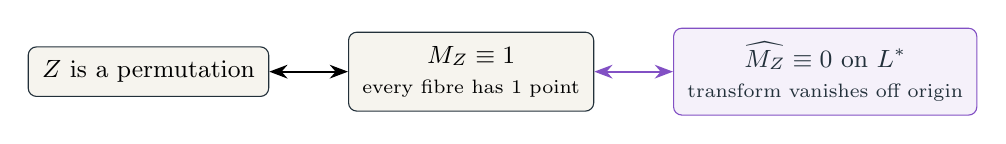
\begin{tikzpicture}[node distance=10mm]
\node[box] (a) {$Z$ is a permutation};
\node[box,right=of a] (b) {$M_Z\equiv 1$\\ \scriptsize every fibre has $1$ point};
\node[fbox,right=of b] (c) {$\widehat{M_Z}\equiv 0$ on $L^\ast$\\ \scriptsize transform vanishes off origin};
\draw[<->,thick] (a)--(b);
\draw[<->,thick,cFour] (b)--(c);
\end{tikzpicture}
\end{center}

\begin{center}\footnotesize
\emph{Lean echoes:}
\texttt{IsDifferenceSet.hasFlatSpectrum},\;
\texttt{KasamiAB.kasami\_is\_ab},\;
\texttt{APNLib.kasami\_isAPN\_diffUnif}.
\end{center}

\vspace{4mm}
% ======================================================================
\section*{3.\quad Hadamard equivalence: slide the spectrum by a power}
% ======================================================================
\noindent\emph{Simple English:} if you already know one flat spectrum, you get a
whole family for free --- just relabel the frequency by a power $t$ that permutes.

\begin{center}
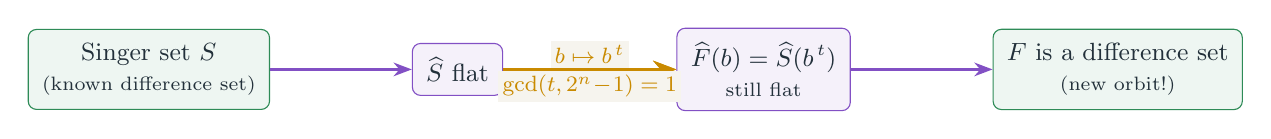
\begin{tikzpicture}[node distance=12mm]
\node[dbox] (S) {Singer set $S$\\ \scriptsize (known difference set)};
\node[fbox,right=18mm of S] (Sh) {$\widehat S$ flat};
\node[fbox,right=22mm of Sh] (Fh) {$\widehat F(b)=\widehat S(b^{\,t})$\\ \scriptsize still flat};
\node[dbox,right=18mm of Fh] (F) {$F$ is a difference set\\ \scriptsize (new orbit!)};

\draw[ar,cFour] (S)--(Sh);
\draw[arb,cGold] (Sh)--(Fh) node[lbl,midway,above]{$b\mapsto b^{\,t}$};
\draw[arb,cGold] (Sh)--(Fh) node[lbl,midway,below]{$\gcd(t,2^n\!-\!1)=1$};
\draw[ar,cFour] (Fh)--(F);
\end{tikzpicture}
\end{center}

\noindent One lemma $\Rightarrow$ three theorems (paper eqns.\ (3)--(5)):
\begin{center}
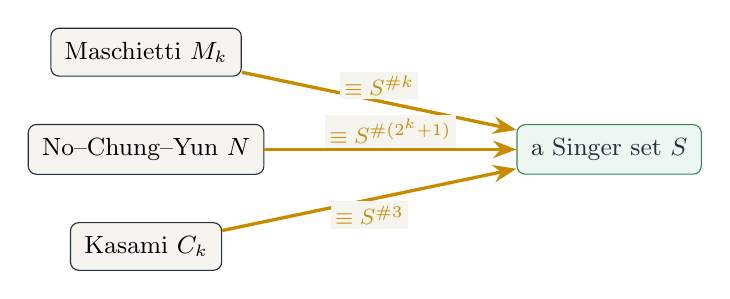
\begin{tikzpicture}[node distance=6mm and 16mm]
\node[box] (M) {Maschietti $M_k$};
\node[box,below=of M] (N) {No--Chung--Yun $N$};
\node[box,below=of N] (C) {Kasami $C_k$};
\node[dbox,right=32mm of N] (Sg) {a Singer set $S$};
\draw[arb,cGold] (M) -- node[lbl,above]{$\equiv S^{\#k}$} (Sg);
\draw[arb,cGold] (N) -- node[lbl,above]{$\equiv S^{\#(2^k+1)}$} (Sg);
\draw[arb,cGold] (C) -- node[lbl,below]{$\equiv S^{\#3}$} (Sg);
\end{tikzpicture}
\end{center}
\begin{center}\footnotesize
Hadamard-equivalence is \emph{coarser} than design equivalence --- that gap is
exactly where the \emph{new} difference sets live.
\end{center}

\newpage
% ======================================================================
\section*{4.\quad Linearize on a torus, then let arithmetic do the work}
% ======================================================================
\noindent\emph{Simple English:} the involution $\zeta\mapsto \zeta+\zeta^{-1}$
turns nonlinear Dickson maps into plain powers on a circle. Then two gcds decide
everything.

\begin{center}
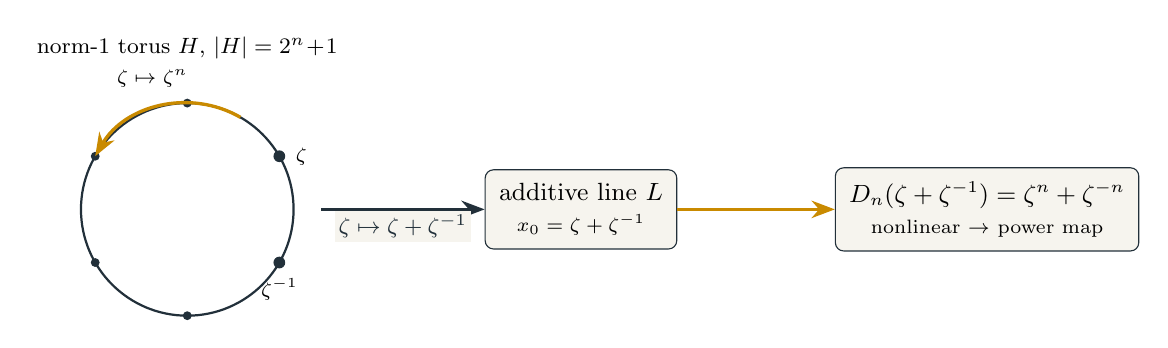
\begin{tikzpicture}
% the torus circle
\begin{scope}[shift={(-4.9,0)}]
  \draw[thick,cInk] (0,0) circle (1.35);
  \node at (0,2.05) {\footnotesize norm-1 torus $H$, $|H|=2^n\!+\!1$};
  \foreach \a in {30,90,150,210,270,330}{\fill[cInk] (\a:1.35) circle (1.6pt);}
  \node[dot,label={[font=\scriptsize]right:$\zeta$}] at (30:1.35) {};
  \node[dot,label={[font=\scriptsize]below:$\zeta^{-1}$}] at (330:1.35) {};
  % power map arrow around circle
  \draw[arb,cGold] (60:1.35) arc (60:150:1.35);
  \node at (105:1.72) {\scriptsize $\zeta\mapsto\zeta^n$};
\end{scope}
% arrow to the line
\node[box] (line) at (0.1,0) {additive line $L$\\ \scriptsize $x_0=\zeta+\zeta^{-1}$};
\draw[arb,cInk] (-3.2,0) -- (line.west)
   node[lbl,midway,below]{$\zeta\mapsto \zeta+\zeta^{-1}$};
% dickson linearizes
\node[box,right=20mm of line] (dick) {$D_n(\zeta+\zeta^{-1})=\zeta^n+\zeta^{-n}$\\ \scriptsize nonlinear $\to$ power map};
\draw[arb,cGold] (line)--(dick);
\end{tikzpicture}
\end{center}

\vspace{1mm}
\noindent\textbf{Fibre sizes reduce to two gcds}, and a rigidity forces them mod 3:
\begin{center}
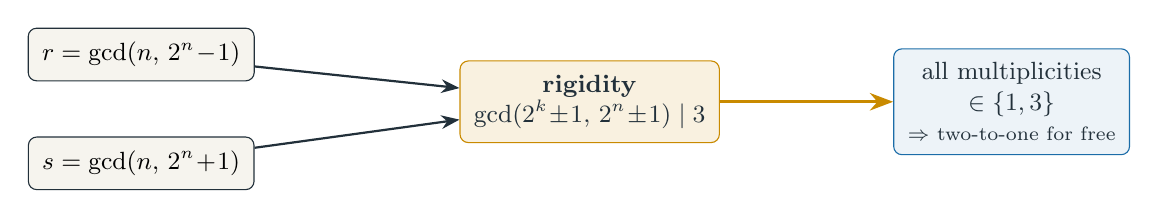
\begin{tikzpicture}[node distance=7mm and 14mm]
\node[box] (r) {$r=\gcd(n,\,2^n\!-\!1)$};
\node[box,below=of r] (s) {$s=\gcd(n,\,2^n\!+\!1)$};
\node[gbox,right=26mm of r,yshift=-6mm] (rig) {\textbf{rigidity}\\ $\gcd(2^k\!\pm\!1,\,2^n\!\pm\!1)\mid 3$};
\node[kbox,right=22mm of rig] (out) {all multiplicities\\ $\in\{1,3\}$\\ \scriptsize $\Rightarrow$ two-to-one for free};
\draw[ar] (r)--(rig);
\draw[ar] (s)--(rig);
\draw[arb,cGold] (rig)--(out);
\end{tikzpicture}
\end{center}

\begin{center}\footnotesize
An entire infinite family collapses to the multiplicity of the tiny
$D_3(X)=X^3+X$: \; $M_{D_{2^k\pm1}}=M_{D_3}$ \; (paper Prop 6 $\to$ Thm 7).
\end{center}

\vspace{2mm}
\begin{center}
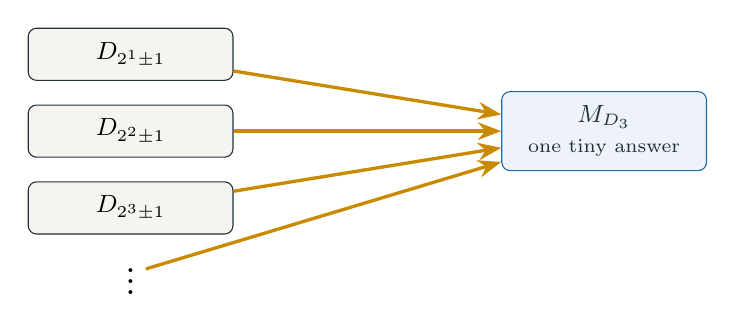
\begin{tikzpicture}[node distance=5mm]
\node[box,minimum width=2.6cm] (f1) {$D_{2^1\pm1}$};
\node[box,minimum width=2.6cm,below=3mm of f1] (f2) {$D_{2^2\pm1}$};
\node[box,minimum width=2.6cm,below=3mm of f2] (f3) {$D_{2^3\pm1}$};
\node[font=\Large,below=1mm of f3] (dots) {$\vdots$};
\node[kbox,right=34mm of f2,minimum width=2.6cm] (d3) {$M_{D_3}$\\ \scriptsize one tiny answer};
\draw[arb,cGold] (f1) -- (d3);
\draw[arb,cGold] (f2) -- (d3);
\draw[arb,cGold] (f3) -- (d3);
\draw[arb,cGold] (dots) -- (d3);
\end{tikzpicture}
\end{center}

\newpage
% ======================================================================
\section*{5.\quad The MCM $\leftrightarrow$ Kasami connection = a square}
% ======================================================================
\noindent\emph{Simple English:} the Kasami derivative is literally the MCM
numerator with an Artin--Schreier glue $t\mapsto t^2+t$ in front. That is a
commuting square.

\begin{center}
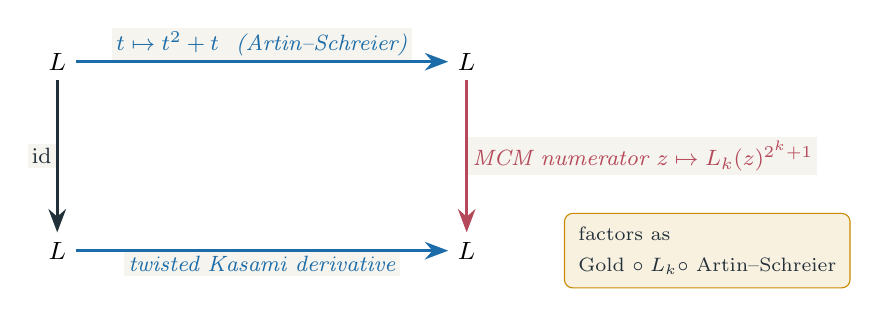
\begin{tikzpicture}[every node/.style={font=\small}]
\node (tl) at (0,2.4) {$L$};
\node (tr) at (5.2,2.4) {$L$};
\node (bl) at (0,0)   {$L$};
\node (br) at (5.2,0) {$L$};
\draw[arb,cKas] (tl)--(tr) node[lbl,midway,above]{$t\mapsto t^2+t$ \ (Artin--Schreier)};
\draw[arb,cInk] (tl)--(bl) node[lbl,midway,left]{$\mathrm{id}$};
\draw[arb,cMcm] (tr)--(br) node[lbl,midway,right]{MCM numerator $z\mapsto L_k(z)^{2^k+1}$};
\draw[arb,cKas] (bl)--(br) node[lbl,midway,below]{twisted Kasami derivative};
\node[gbox,right=10mm of br,align=left] {\scriptsize
  factors as\\ \scriptsize Gold $\circ\;L_k\circ$ Artin--Schreier};
\end{tikzpicture}
\end{center}
\begin{center}\footnotesize
Key identity: \;
$\bigl((t+1)^{\dk}+t^{\dk}+1\bigr)\,(t^2+t)^{2^k}=(t^{2^k}+t)^{2^k+1}$.\\
\emph{Lean:} \texttt{MCMKasamiCat.mcmKasami\_commSq},\;
\texttt{...\,mcmNumerator\_comp\_artinSchreier}.
\end{center}

\vspace{3mm}
% ======================================================================
\section*{6.\quad Three symmetries of the parameter $k$}
% ======================================================================
\noindent\emph{Simple English:} the exponent $\dk$ can be moved three ways. Each
move keeps the property you care about. They are different arrows in \emph{one}
equivalence groupoid.

\begin{center}
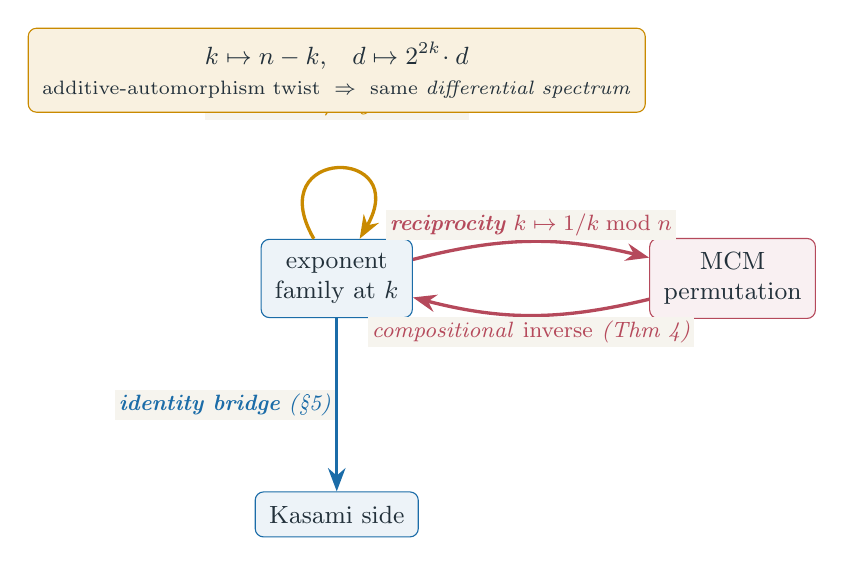
\begin{tikzpicture}
\node[kbox] (k) at (0,0) {exponent\\ family at $k$};
% frobenius loop
\draw[arb,cGold] (k) to[out=120,in=60,loop,looseness=6]
   node[lbl,above=6mm]{\textbf{Frobenius / cyclotomic}} (k);
\node[gbox,above=16mm of k] (fr) {$k\mapsto n-k$,\quad $d\mapsto 2^{2k}\!\cdot d$\\
   \scriptsize additive-automorphism twist $\;\Rightarrow\;$ same \emph{differential spectrum}};
% reciprocity
\node[mbox,right=30mm of k] (kk) {MCM\\ permutation};
\draw[arb,cMcm] (k) to[bend left=14] node[lbl,above]{\textbf{reciprocity} $k\mapsto 1/k \bmod n$} (kk);
\draw[arb,cMcm] (kk) to[bend left=14] node[lbl,below]{compositional \emph{inverse} (Thm 4)} (k);
% identity bridge
\node[kbox,below=22mm of k] (br) {Kasami side};
\draw[arb,cKas] (k) -- node[lbl,left]{\textbf{identity bridge} (\S5)} (br);
\end{tikzpicture}
\end{center}

\begin{center}\footnotesize
\renewcommand{\arraystretch}{1.3}
\begin{tabular}{@{}l l l l@{}}
\hline
\textbf{move} & \textbf{on $k$} & \textbf{on exponent} & \textbf{preserves}\\
\hline
Frobenius / cyclotomic & $k\mapsto n-k$ & $d\mapsto 2^{2k}d$ & differential spectrum (APN/AB)\\
MCM$\leftrightarrow$Kasami (Thm 4) & $k\mapsto 1/k$ & multiplicative inverse & permutation-ness\\
identity bridge (Cor 2) & --- & Artin--Schreier glue & the $2$-to-$1$ count\\
\hline
\end{tabular}
\end{center}

\begin{center}\footnotesize
The Frobenius move is the paper's one-line WLOG ``replace $k$ by $n-k$ if $k$ is
even; this does not change the APN property''. \emph{Lean:}
\texttt{FrobeniusGroupoid.kasamiComplementIso},\;
\texttt{...\,diffUnifFunctor}.
\end{center}

\newpage
% ======================================================================
\section*{7.\quad How the patterns propagate through the paper}
% ======================================================================
\noindent\emph{Simple English:} read top to bottom. Each box uses the pattern
above it. Colour = which structural idea is doing the work.

\begin{center}
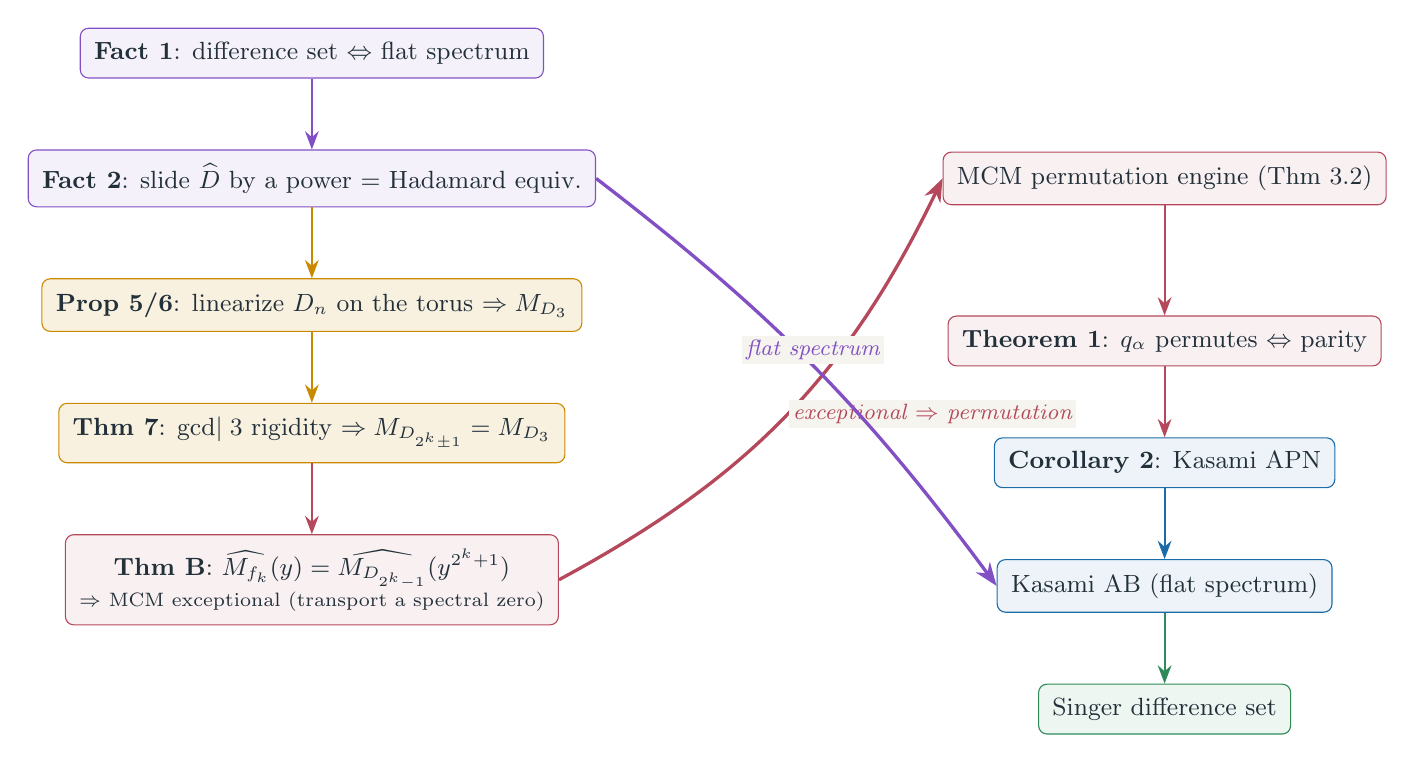
\begin{tikzpicture}[node distance=9mm,every node/.style={font=\small}]
\node[fbox] (f1) {\textbf{Fact 1}: difference set $\Leftrightarrow$ flat spectrum};
\node[fbox,below=of f1] (f2) {\textbf{Fact 2}: slide $\widehat D$ by a power $=$ Hadamard equiv.};
\node[gbox,below=of f2] (p6) {\textbf{Prop 5/6}: linearize $D_n$ on the torus $\Rightarrow M_{D_3}$};
\node[gbox,below=of p6] (t7) {\textbf{Thm 7}: gcd$\mid 3$ rigidity $\Rightarrow M_{D_{2^k\pm1}}=M_{D_3}$};
\node[mbox,below=of t7] (tb) {\textbf{Thm B}: $\widehat{M_{f_k}}(y)=\widehat{M_{D_{2^k-1}}}(y^{2^k+1})$\\
   \scriptsize $\Rightarrow$ MCM exceptional (transport a spectral zero)};

% right column: the APN spine
\node[mbox,right=44mm of f2] (eng) {MCM permutation engine (Thm 3.2)};
\node[mbox,below=14mm of eng] (t1) {\textbf{Theorem 1}: $q_\alpha$ permutes $\Leftrightarrow$ parity};
\node[kbox,below=of t1] (c2) {\textbf{Corollary 2}: Kasami APN};
\node[kbox,below=of c2] (ab) {Kasami AB (flat spectrum)};
\node[dbox,below=of ab] (ds) {Singer difference set};

\draw[ar,cFour] (f1)--(f2);
\draw[ar,cGold] (f2)--(p6);
\draw[ar,cGold] (p6)--(t7);
\draw[ar,cMcm]  (t7)--(tb);

\draw[ar,cMcm] (eng)--(t1);
\draw[ar,cMcm] (t1)--(c2);
\draw[ar,cKas] (c2)--(ab);
\draw[ar,cDs]  (ab)--(ds);

\draw[arb,cMcm] (tb.east) to[bend right=18]
   node[lbl,right]{exceptional $\Rightarrow$ permutation} (eng.west);
\draw[arb,cFour] (f2.east) to[bend left=8]
   node[lbl,above]{flat spectrum} (ab.west);
\end{tikzpicture}
\end{center}

\vspace{4mm}
\begin{center}\footnotesize
\renewcommand{\arraystretch}{1.35}
\begin{tabular}{@{}l l l@{}}
\hline
\textbf{pattern} & \textbf{where} & \textbf{what it buys}\\
\hline
\textcolor{cFour}{Fourier duality} & Facts 1--2, Thm B & geometry $\to$ transform identity\\
\textcolor{cGold}{Hadamard equivalence} & Fact 2, eqns (3)--(5) & one lemma $\to$ many difference sets; new orbits\\
\textcolor{cGold}{linearize on a torus} & Prop 5/6 & fibre sizes $=$ two gcds\\
\textcolor{cGold}{gcd $\mid 3$ rigidity} & Thm 7 & infinite family shares $M_{D_3}$\\
\textcolor{cInk}{multiplicity trichotomy} & before Thm B & uniform ``is a permutation'' test\\
\hline
\end{tabular}
\end{center}

\vfill
\begin{center}\footnotesize
\parbox{0.88\textwidth}{\centering
\textbf{One sentence.} Every hard multiplicative property is dragged to the
Fourier side, where it becomes a \emph{flatness} or a \emph{vanishing}, and is
then carried between objects by \emph{power-permutation reparametrization} ---
with Dickson maps linearized on a torus and a $\gcd\mid 3$ rigidity forcing all
the multiplicities into line.}
\end{center}

\end{document}
